\section*{HOW TO}
This template is used for the workshop reports of the \coursename\ course. Remove this section by editing the \texttt{reportContent.tex} file \textbf{after} you have understood how to use this template.

\subsection*{Folder Structure}
\begin{lstlisting}[escapechar=!]
WorkshopReport /
  |- reportContent /  <-- YOUR working folder
      |- images /     <-- Images are stored here
      |- sections /   <-- Additional sections / tex-files here
          |- _HOWTO_.tex    <-- *this* How To section
          |- introduction.tex
          |- lessons-learned.tex
          '- section2.tex
      '- reportContent.tex  <-- Change your section imports here
  |- !\rootDocument!  <-- DO NOT alter this file
  |- llncs.cls                            <-- NOR that
  |- splncs03.bst                         <-- NOR that
  '- UniBas_Logo_EN_Schwarz_RGB_65.pdf    <-- NOR that
\end{lstlisting}
\ 

\subsection*{Setup}
Your report is compiled using the \texttt{\rootDocument} file. Therefore, we suggest that you set the file \texttt{\rootDocument} as the Master-/Root-Document that you can conveniently work on your report. 


\subsection*{Images}
Images placed in the \texttt{images} sub-folder can be used directly in the \texttt{\textbackslash includegraphics} command -- see also \Cref{fig:rosette}. Also, sub-figures are possible: \Cref{fig:fly,fig:flies}.

Please \textsc{do~not} store your images elsewhere! 

\begin{figure}[tb]
\centering
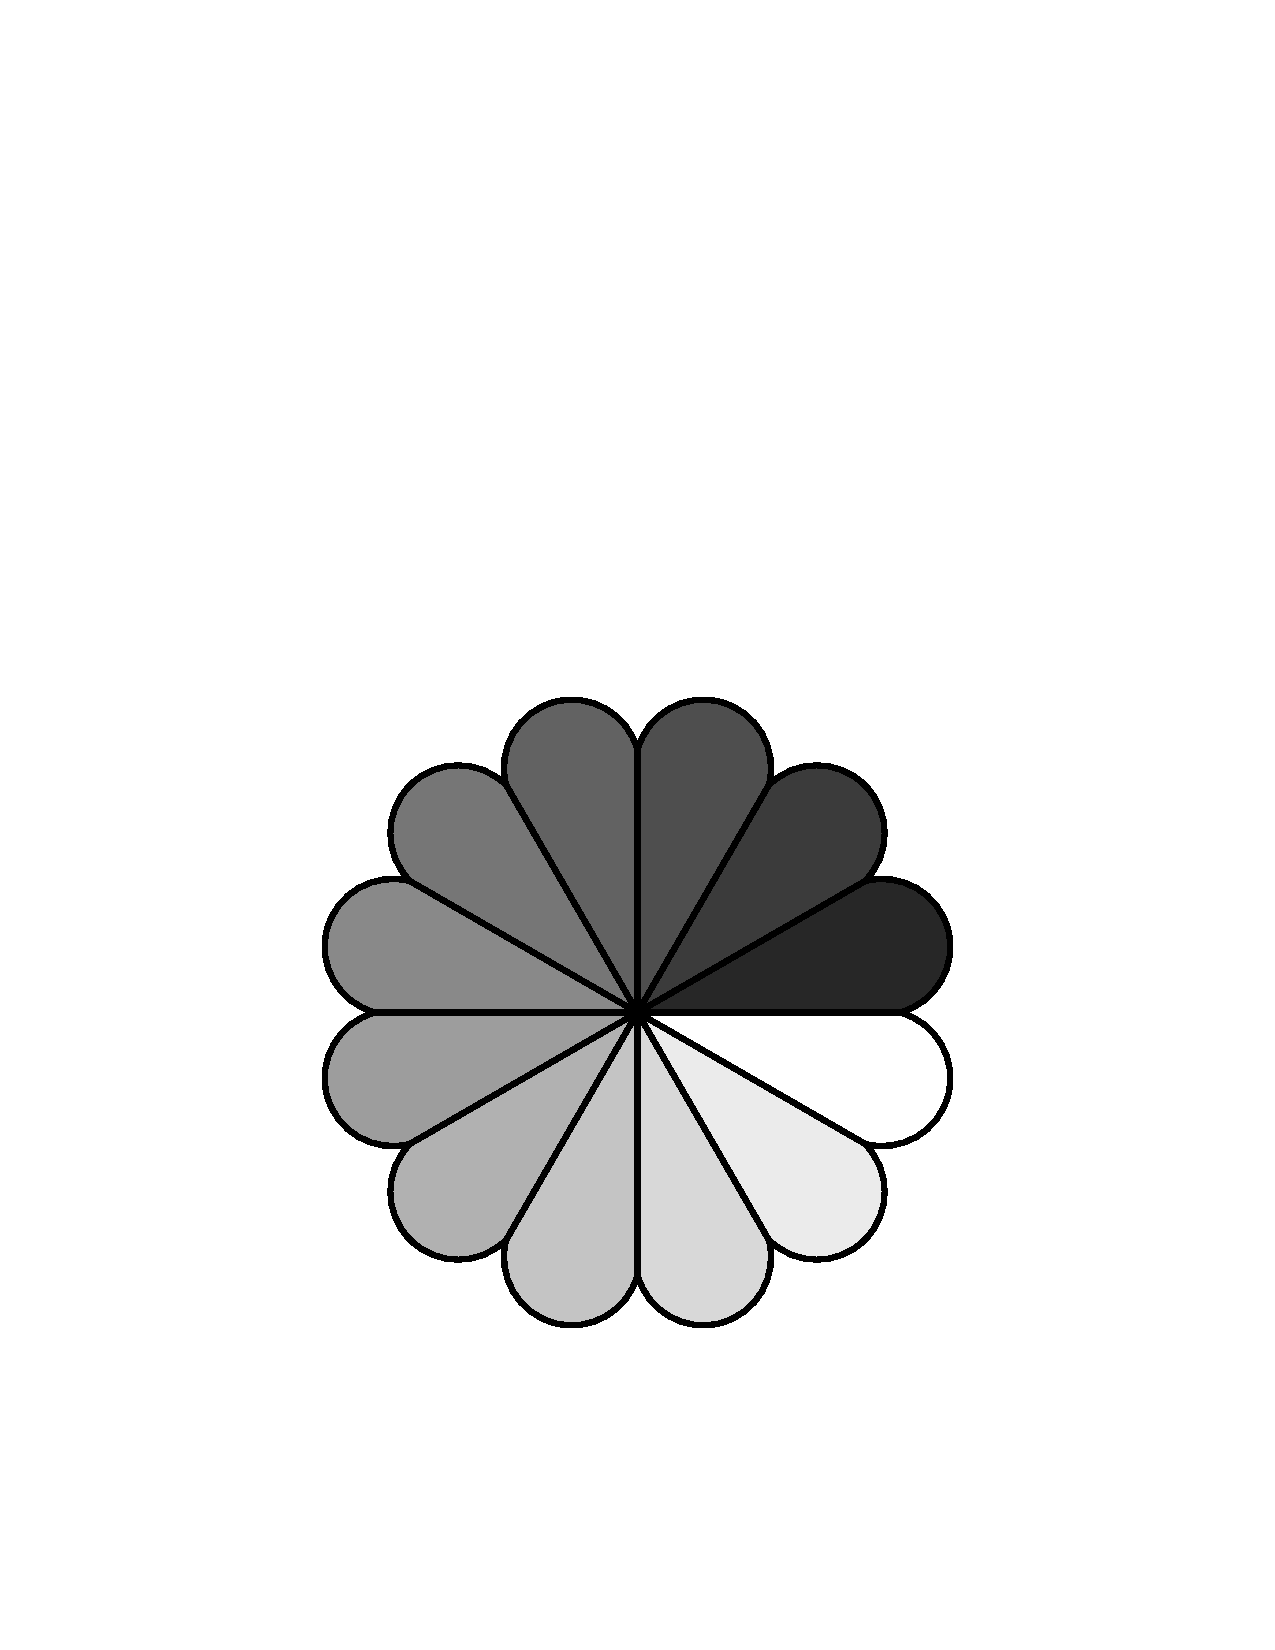
\includegraphics[width=0.45\textwidth]{rosette}
\caption{Example figure stored in the \texttt{images} sub-folder and displayed with \texttt{\textbackslash includegraphics[width=0.45\textbackslash textwidth]\{rosette\}}}
\label{fig:rosette}
\end{figure}

\begin{figure}[tb]
\centering
    %\subfloat[CAPTION]{BILDERCODE}\qquad
    \subfloat[A fly\label{fig:fly}]{
\includegraphics[width=0.4\textwidth]{fly}}\qquad
    \subfloat[Flies\label{fig:flies}]{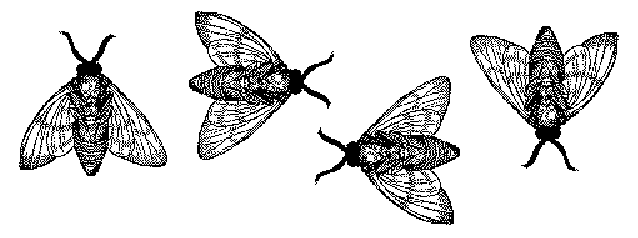
\includegraphics[width=0.45\textwidth]{flies}}
\caption{Example figure stored in the \texttt{images} sub-folder}
\label{fig:example subfigure}
\end{figure}


\subsection*{Code}
To illustrate code use the \texttt{lstlisting} environment:
\begin{lstlisting}[language=Java]
public void foo( final int bar ) {
  System.out.println( bar );
}
\end{lstlisting}


\subsection*{References}
Your references are stored in the \texttt{reportContent.tex} file and used with the \texttt{\textbackslash cite} command. For example: \cite{IEEEhowto:kopka}.

Unfortunately, you cannot use a bibliography generated by BibTeX as a .bbl file directly. Use \texttt{\textbackslash bibliographystyle\{IEEEtran\}} and \texttt{\textbackslash bibliography\{references\}} (the argument is your BibTeX string definitions and bibliography database(s), e.\,g. \texttt{references.bib}) along with all \texttt{\textbackslash cite} commands in a separate \texttt{tex} document to generate a .bbl file using BibTeX. Then, copy manually the resultant .bbl file content into the \texttt{thebibliography} environment in the \texttt{reportContent.tex} file. Also, set the second argument of the \texttt{\textbackslash begin} to the number of references (used to reserve space for the reference number labels box).

\pagebreak